\documentclass{article}
\usepackage[utf8]{inputenc}
%Header Dimensions
%https://tex.stackexchange.com/questions/40183/problem-with-the-header-footer-width#40184
\usepackage[margin=0.5in,bottom=0.5in,top=0.5in]{geometry}

\usepackage{graphicx}
\usepackage{float}

\usepackage{caption}
\usepackage{subcaption}

\usepackage{listings}

\title{Homework 3 - CS317 Spring 2019}
\author{Matt Fletcher}
\begin{document}
\maketitle

\begin{enumerate}

%Q1
\item The goal of dynamic programming is to create polynomial time solutions to problems by holding solutions to previous subproblems in a table to be re-used in future uses of that subproblem. A problem is said to have overlapping subproblems if it can be broken down into subproblems which are used multiple times. Optimal substructure is when the globally optimal solution can be constructed from locally optimal solutions to subproblems.
    
    The four steps to dynamic programming approach are:

\begin{enumerate}
	\item Characterize the structure of an optimal solution. 
	
	\item Recursively define the value of an optimal solution by expressing the solution of the original problem in terms of optimal solutions for smaller problems. 

	\item Bottom up computation, compute the value of an optimal solution in a bottom-up fashion by using a table structure. 

	\item Construct the optimal solution by expressing the solution of the original problem in terms of optimal solutions for smaller subproblems. 
	 
\end{enumerate}

\noindent\rule{8cm}{0.4pt}

%Q2 Matrix Chain Multiplication 
\item  
    \begin{enumerate}
        \item Step 1 is finding the optimal substructure and using it to construct an optimal solution to the subproblems. By finding an optimal parenthesization of a subset of the matrices, we can use that subset to find an optimal parenthensization of the full set of matrices. 

        \item Now, define the cost of an optimal solution recursively in terms of the optimal solution to subproblems. 

        \item Compute the optimal costs. Without dynamic programming, this algorithm would take exponential time. We can compute the optimal costs using a tabular method. 
            The Matrix Chain order defined in the text results in an $O(n^3)$ algorithm instead of an exponential algorithm that would result from a brute force approach. 

        \item The Matrix Chain order defined in the previous problem determines the number of multiplications required but not directly how to multiply them.  The table produced gives us the required information. 
    \end{enumerate}
\noindent\rule{8cm}{0.4pt}


%Q3 Longest Common Subsequence
\item  
    
    \begin{enumerate}
        \item A brute force solution to this problem would result in an exponential algorithm. The LCS problem has an optimal substructure property, however. In other words, a solution to a subproblem can be re-used in further steps. 
            

        \item The recursive solution to the LCS problem involves establishing a recurrence for the value of an optimal solution. This is the LCS of $X_{i-1}$ and $Y_{i-1}$ if the two characters at matching locations are equal. Otherwise, find the LCS of $X$ and $Y_{i-1}$. 

        \item The algorithm takes 2 sequences $X$ and $Y$ and stored them in a table. This table is filled out in row-major order. Each cell in the table points to the table entry containing the optimal subproblem solution. This allows a solution to be found after filling out the table.
            

        \item  The table filled with the arrows allows for a constrcution of the LCS. Trace through the table following the arrows, and whenever a diagonal arrow is encountered, it implied that that particular row/column is a solution of the LCS. Hence, a solution is easily found. 
            
    \end{enumerate}

    TODO TODO TODO TODO TODO 
    TODO finish in spreadsheet.

\noindent\rule{8cm}{0.4pt}

%Q4 Floyds
\item 
Begin by visualizing the graph. 

\begin{figure}[H]
	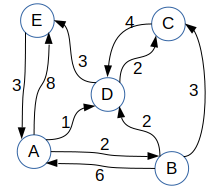
\includegraphics[]{P4/graph}
\end{figure}

Now, write the beginning table. 
\begin{table}[H]
\begin{tabular}{|l|l|l|l|l|l|}
\hline
 & A & B & C & D & E \\ \hline
A & 0 & 2 & $\infty$ & 1 & 8 \\ \hline
B & 6 & 0 & 3 & 2 & $\infty$ \\ \hline
C & $\infty$ & $\infty$ & 0 & 4 & $\infty$ \\ \hline
D & $\infty$ & $\infty$ & 2 & 0 & 3 \\ \hline
E & 3 & $\infty$ & $\infty$ & $\infty$ & 0 \\ \hline
\end{tabular}
\end{table}

Update the table by seeing if any paths are shortened by going through A. 

\begin{table}[H]
\begin{tabular}{|l|l|l|l|l|l|}
\hline
 & A & B & C & D & E \\ \hline
A & 0 & 2 & $\infty$ & 1 & 8 \\ \hline
B & 6 & 0 & 3 & 2 & 14 \\ \hline
C & $\infty$ & $\infty$ & 0 & 4 & $\infty$ \\ \hline
D & $\infty$ & $\infty$ & 2 & 0 & 3 \\ \hline
E & 3 & 5 & $\infty$ & 4 & 0 \\ \hline
\end{tabular}
\end{table}

Now do the same through B. 
\begin{table}[H]
\begin{tabular}{|l|l|l|l|l|l|}
\hline
 & A & B & C & D & E \\ \hline
A & 0 & 2 & 5 & 1 & 8 \\ \hline
B & 6 & 0 & 3 & 2 & 14 \\ \hline
C & $\infty$ & $\infty$ & 0 & 4 & $\infty$ \\ \hline
D & $\infty$ & $\infty$ & 2 & 0 & 3 \\ \hline
E & 3 & 5 & $\infty$ & 4 & 0 \\ \hline
\end{tabular}
\end{table}

Node C: Nothing is optimized, table is unchanged. 

\begin{table}[H]
\begin{tabular}{|l|l|l|l|l|l|}
\hline
 & A & B & C & D & E \\ \hline
A & 0 & 2 & 5 & 1 & 8 \\ \hline
B & 6 & 0 & 3 & 2 & 14 \\ \hline
C & $\infty$ & $\infty$ & 0 & 4 & $\infty$ \\ \hline
D & $\infty$ & $\infty$ & 2 & 0 & 3 \\ \hline
E & 3 & 5 & $\infty$ & 4 & 0 \\ \hline
\end{tabular}
\end{table}



\begin{table}[H]
\begin{tabular}{|l|l|l|l|l|l|}
\hline
 & A & B & C & D & E \\ \hline
A & 0 & 2 & 3 & 1 & 4 \\ \hline
B & 6 & 0 & 3 & 2 & 5 \\ \hline
C & $\infty$ & $\infty$ & 0 & 4 & 7 \\ \hline
D & $\infty$ & $\infty$ & 2 & 0 & 3 \\ \hline
E & 3 & 5 & 6 & 4 & 0 \\ \hline
\end{tabular}
\end{table}


\begin{table}[H]
\begin{tabular}{|l|l|l|l|l|l|}
\hline
 & A & B & C & D & E \\ \hline
A & 0 & 2 & 3 & 1 & 4 \\ \hline
B & 6 & 0 & 3 & 2 & 5 \\ \hline
C & 10 & 12 & 0 & 4 & 7 \\ \hline
D & 6 & 8 & 2 & 0 & 3 \\ \hline
E & 3 & 5 & 6 & 4 & 0 \\ \hline
\end{tabular}
\end{table}



\noindent\rule{8cm}{0.4pt}

%Q5 Knapsack Question
\item The knapsack problem is as follows: "Given n items of weights $w_i$ and values $v_j$, and a knapsack of capacity W, find the most valuable subset of the items that fit into the knapsack. The dynamic approach to solving the knapsack problem consists of breaking the set of all the subsets of the first $i$ items that fit the knapscak of capacity $J$ into 2 categories: those that do not include the $i^{th}$ item and those that do. 

Use a table to reduce the number of recalculations needed.

\begin{table}[H]
\begin{tabular}{|l|l|l|l|l|l|l|l|}
\hline
 & 0 & 1 & 2 & 3 & 4 & 5 & 6 \\ \hline
0 & 0 & 0 & 0 & 0 & 0 & 0 & 0 \\ \hline
1 & 0 & 0 & 0 & 25 & 25 & 25 & 25 \\ \hline
2 & 0 & 0 & 20 & 25 & 25 & 45 & 45 \\ \hline
3 & 0 & 15 & 20 & 35 & 40 & 45 & 45 \\ \hline
4 & 0 & 15 & 20 & 35 & 40 & 55 & 60 \\ \hline
5 & 0 & 15 & 20 & 35 & 40 & 55 & 65 \\ \hline
\end{tabular}
\end{table}

Items 3 and 5 will create the optimal solution of \$65 in the knapsack. TODO CHECK  

\noindent\rule{8cm}{0.4pt}

%Q6 P NP
\item Class P problems are those that have a polynomial time solution. This includes problems such as sorting a list or finding the largest element. Problems in class NP have non-polynomial time solutions but are able to be checked in polynomial time. For example, the traveling salesman problem problem only can be solved in non-polynomial time. The P-NP problem asks whether every problem which has a solution that can be checked in polynomial time also has a solution that can be solved in polynomial time. If P is shown to be equal to NP, then one major effect will be that modern RSA encryption will be easily able to be broken, given that RSA encryption relies on a solution only being able to be found in NP time. 

\noindent\rule{8cm}{0.4pt}


%Q7 Backtracking, N-Queens
\item 

    The backtracking technique is stopping a particular branch when a solution using that appproach is no longer possible. In the N-Queens problem, n queens must be places on an n $\times$ n board such that no 2 queens are in the same row, column, or diagonal. To use backtracking, stop attempting to solve a board when it is impossible for the next queen to be placed. 

    \begin{table}[H]
        \begin{tabular}{|l|l|l|l|}
        \hline
        Q & - & - & - \\ \hline
        | & \textbackslash{} &  &  \\ \hline
        | &  & \textbackslash{} &  \\ \hline
        | &  &  & \textbackslash{} \\ \hline
        \end{tabular}
    \end{table}

\begin{table}[H]
\begin{tabular}{|l|l|l|l|}
\hline
Q & - & - & - \\ \hline
| & \textbackslash{} & Q & - \\ \hline
| & / & \textbackslash{} & \textbackslash{} \\ \hline
| &  & | & \textbackslash{} \\ \hline
\end{tabular}
\end{table}


Not enough squares remain. Go back and try the next square for queen 2. 

\begin{table}[H]
\begin{tabular}{|l|l|l|l|}
\hline
Q & - & - & - \\ \hline
| & \textbackslash{} & - & Q \\ \hline
| &  & \textbackslash{} & | \\ \hline
| & / &  & \textbackslash{} \\ \hline
\end{tabular}
\end{table}


\begin{table}[H]
\begin{tabular}{|l|l|l|l|}
\hline
Q & - & - & - \\ \hline
| & \textbackslash{} & - & Q \\ \hline
| & Q & \textbackslash{} & | \\ \hline
| & / & \textbackslash{} & \textbackslash{} \\ \hline
\end{tabular}
\end{table}

Not enough squares remain. Go back to the first queen and try the next square. 

\begin{table}[H]
\begin{tabular}{|l|l|l|l|}
\hline
- & Q & - & - \\ \hline
/ & | & \textbackslash{} &  \\ \hline
 & | &  & \textbackslash{} \\ \hline
 & | &  &  \\ \hline
\end{tabular}
\end{table}


\begin{table}[H]
\begin{tabular}{|l|l|l|l|}
\hline
- & Q & - & - \\ \hline
/ & | & \textbackslash{} & Q \\ \hline
 & | & / & \textbackslash{} \\ \hline
 & | &  & | \\ \hline
\end{tabular}
\end{table}


\begin{table}[H]
\begin{tabular}{|l|l|l|l|}
\hline
- & Q & - & - \\ \hline
/ & | & \textbackslash{} & Q \\ \hline
Q & | & / & \textbackslash{} \\ \hline
| & | &  & | \\ \hline
\end{tabular}
\end{table}


\begin{table}[H]
\begin{tabular}{|l|l|l|l|}
\hline
- & Q & - & - \\ \hline
/ & | & \textbackslash{} & Q \\ \hline
Q & | & / & \textbackslash{} \\ \hline
| & | & Q & | \\ \hline
\end{tabular}
\end{table}

As all 4 queens have been placed, and no 2 are in the same row, column, or diagonal, this is the final solution to the problem. 





\noindent\rule{8cm}{0.4pt}

%Q8 Branch and Bound
\item Begin by sorting the table on the weight/value ratio. 

\begin{table}[H]
\begin{tabular}{|l|l|l|l|}
\hline
Item & Weight & Value & Val/Weight \\ \hline
1 & 3 & 30 & 10 \\ \hline
2 & 6 & 42 & 7 \\ \hline
3 & 2 & 10 & 5 \\ \hline
4 & 3 & 15 & 5 \\ \hline
\end{tabular}
\end{table}


%TODO FINISH
\begin{figure}[H]
        \centering
	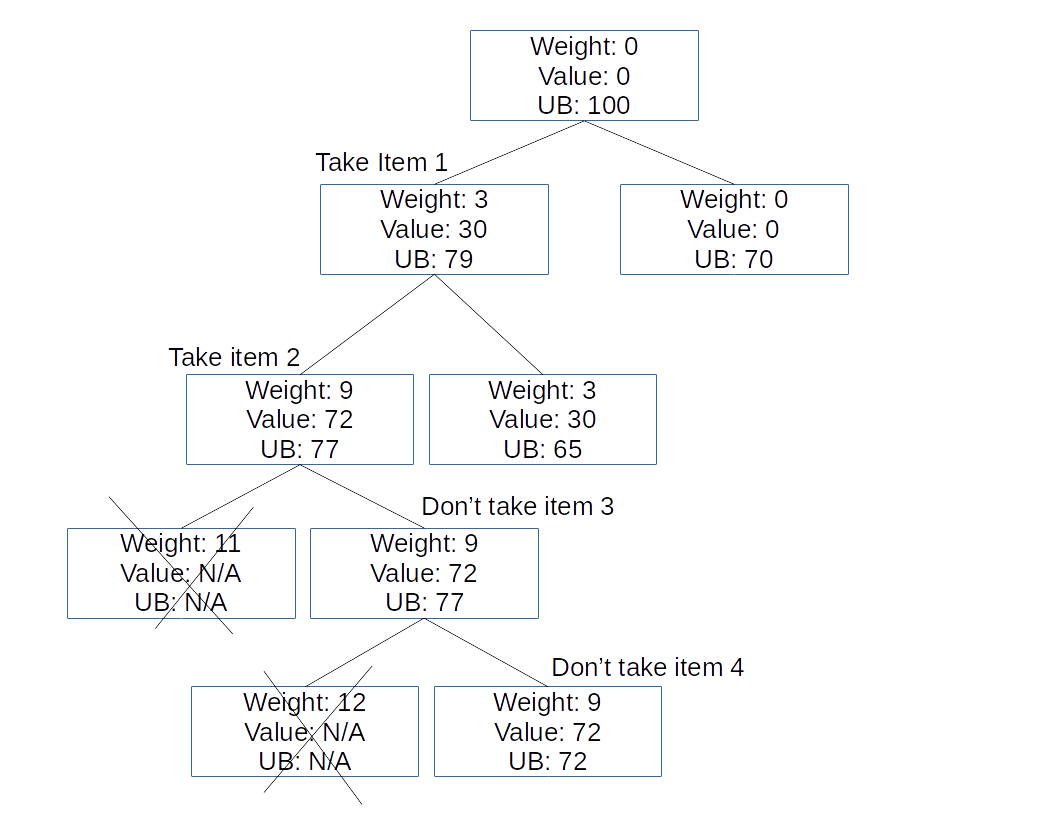
\includegraphics[width=0.7\textwidth]{P8/branchandbound}
\end{figure}

Therefore, the optimal solution takes items 1 and 2, with a value of 72. 

\noindent\rule{8cm}{0.4pt}

%Q9 Huffman Encoding 
\item The following table contains the output of a huffman encoder written in Python. TODO finish.
\begin{lstlisting}
 Char | Freq  | Huffman code
-----------------------------
 'i'  |     7 |           10
 't'  |     3 |          010
 'o'  |     2 |          000
 'n'  |     2 |         0111
 'a'  |     2 |         0110
 'b'  |     2 |         1101
 'u'  |     2 |         1100
 'h'  |     1 |         0010
 'r'  |     1 |        00111
 'f'  |     1 |        00110
 'c'  |     1 |        11101
 'l'  |     1 |        11100
 'd'  |     1 |        11111
 's'  |     1 |        11110

\end{lstlisting}

\noindent\rule{8cm}{0.4pt}


%Q10 BST
\item 
The following images show the construction of a binary search tree given the input list. 

\begin{figure}[H]
	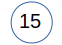
\includegraphics[]{P10/0-15}
	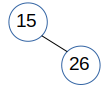
\includegraphics[]{P10/1-26}
	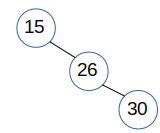
\includegraphics[]{P10/2-30}
	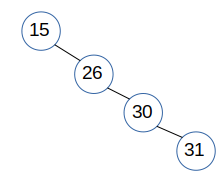
\includegraphics[]{P10/3-31}
	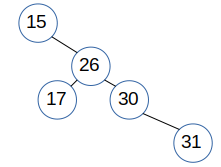
\includegraphics[]{P10/4-17}
	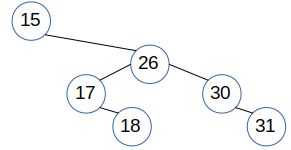
\includegraphics[]{P10/5-18}
	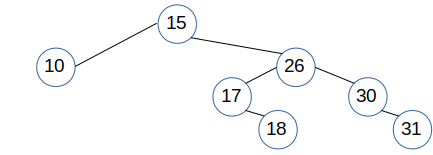
\includegraphics[]{P10/6-10}
	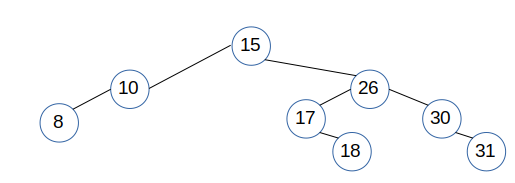
\includegraphics[]{P10/7-8}
\end{figure}

\begin{figure}[H]
	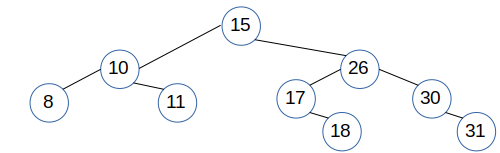
\includegraphics[]{P10/8-11}
	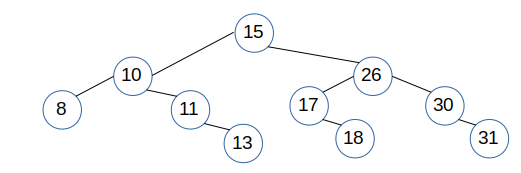
\includegraphics[]{P10/9-13}
	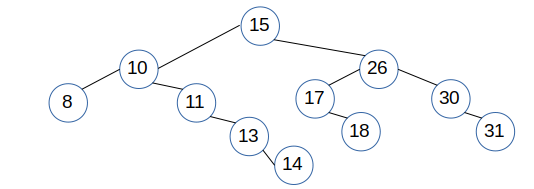
\includegraphics[]{P10/10-14}
	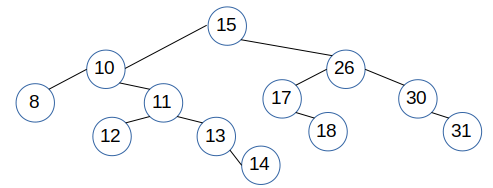
\includegraphics[]{P10/11-12}
\end{figure}

A BST insertion and deletion is least optimal when the input list is ordered. This turns the tree from a binary tree into a linked list. This changes the efficiency from $O(\log n)$ to $O(n)$. A worst case input would be $1,2,3,4,5$. 

\noindent\rule{8cm}{0.4pt}


%Q9 BST deletion
\item
Here is the original tree. 

\begin{figure}[H]

	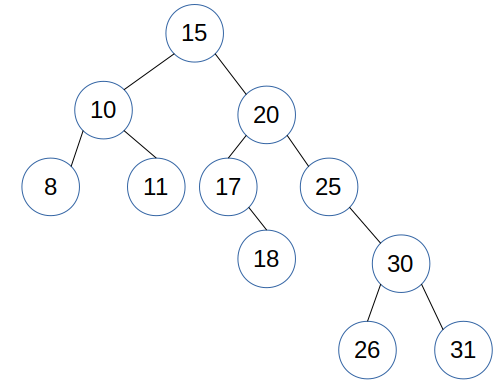
\includegraphics[width=0.7\textwidth]{P11/full}
\end{figure}



We wish to delete node \#20. Because it has 2 children, we find the largest element in the left subtree, swap it with 20, and then delete that node. 
 
\begin{figure}[H]
	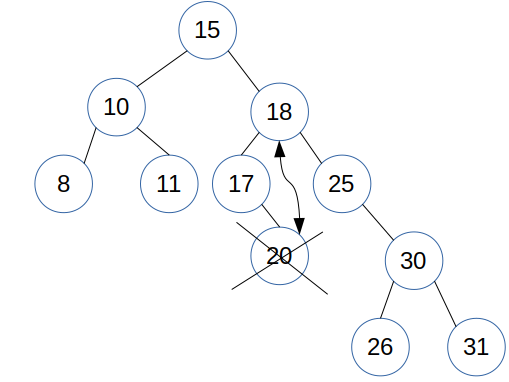
\includegraphics[width=0.7\textwidth]{P11/20}
\end{figure}


Now, we wish to delete node \#25. Because it only has 1 child, we simply point the parent node to point towards the child of \#25, as shown in the figure below: 

\begin{figure}[H]
	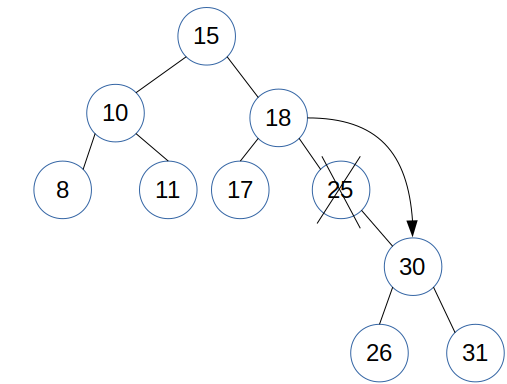
\includegraphics[width=0.7\textwidth]{P11/25}
\end{figure}

In the end, the tree looks as follows:

\begin{figure}[H]
	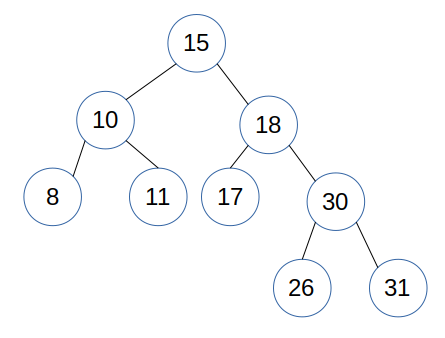
\includegraphics[width=0.7\textwidth]{P11/final}
\end{figure}
\noindent\rule{8cm}{0.4pt}


\end{enumerate}




\end{document}
